\section{Implémentation}

L’implémentation du logiciel a été réalisée par étapes, en suivant les \textit{job stories} décrites dans la \autoref{sec:features} ainsi que les tâches planifiées dans le diagramme de Gantt présenté en \autoref{fig:gantt_prototype_phases_detailed}.

La \autoref{fig:structure_interactions} illustre l’architecture logicielle globale ainsi que les interactions entre les deux projets (client et robot).

\begin{figure}[H]
    \centering
    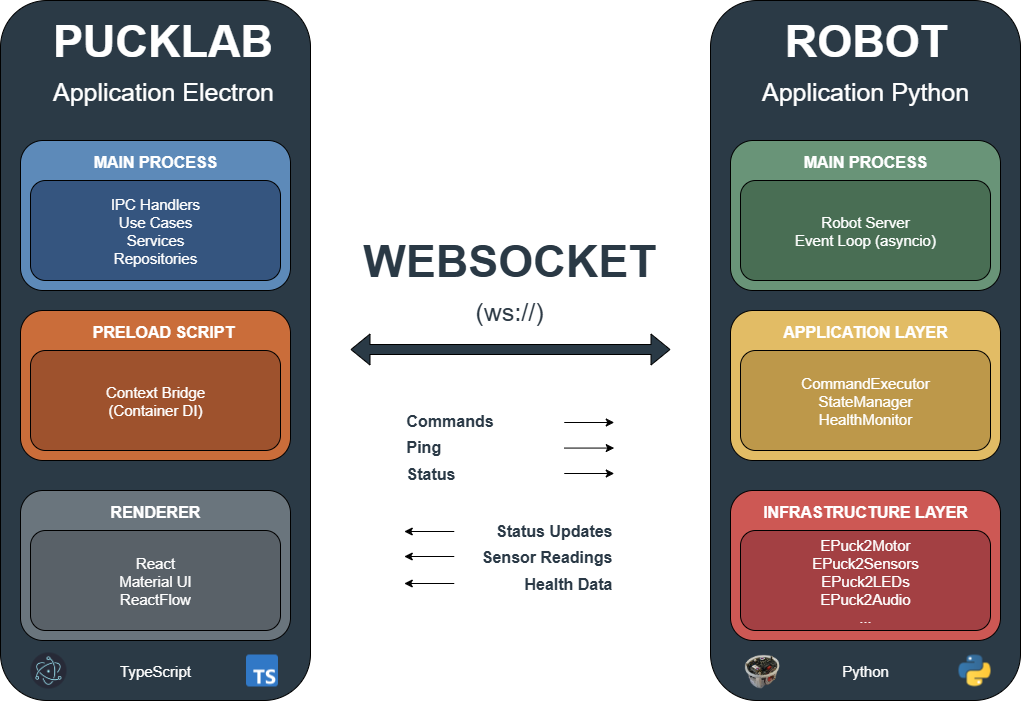
\includegraphics[width=1\linewidth]{.//figures//implementation-schema.png}
    \caption{\label{fig:structure_interactions} Structure et interactions des codebases}
\end{figure}

\subsection{Développement de l'interface utilisateur (client)}

La première phase a porté sur le développement de l’interface utilisateur avec Electron, en s’appuyant sur React comme moteur de rendu, et sur le langage TypeScript pour bénéficier d’un typage fort assurant une meilleure robustesse du code.

Une attention particulière a été portée à l’implémentation de la \textit{clean architecture}, afin de bien distinguer les responsabilités entre les différentes couches applicatives et leur contexte d’exécution.
En effet, Electron repose sur une séparation stricte entre le \textit{main process} (responsable de la gestion des fenêtres, du système de fichiers, etc.) et le \textit{renderer process} (dédié à l’affichage de l’interface).
Ces deux processus ne pouvant pas interagir directement, un pont de communication a été mis en place via un \textit{context bridge}, étendant l’objet global $Window$ pour exposer une API sécurisée entre les deux contextes.

Une fois cette structure maîtrisée, le développement de l’interface a pu se poursuivre de manière fluide.

\subsection{Développement du firmware embarqué (robot)}

La seconde phase de développement a concerné le \textit{firmware}, conçu comme un serveur Python s’exécutant sur le Raspberry Pi du robot e-puck2. 
Ce serveur établit une communication bidirectionnelle via WebSocket avec l’interface Electron, exécute les commandes reçues, et transmet les états et données du robot en retour.

Là encore, une architecture en couches a été définie selon les principes de la \textit{clean architecture}, en séparant clairement les responsabilités entre la couche \textit{domaine}, la couche \textit{application}, et la couche \textit{infrastructure} en lien direct avec le matériel (moteurs, capteurs, LEDs, etc.).
